\scanpage{69}
\mspage{30}
\uline{propriété universelle} évidente pour les morphismes
de \unsure{\unsure{cette|la}|\deleted{\unsure{cette|la}}} categorie topologique $\uline{\Sigma}$ dans un ens. \inserted{pré}ordonné.
\S\ Supposons maintenant que $\uline{\Sigma}$ satisfasse les
% The two drafts below are cancelled by the actual stepped outline and
% three oblique strokes. Their running letters remain typeset text.
% No additional horizontal strike rules are supplied inside this drawing.
\figure{
\begin{tikzpicture}[x=1cm,y=-1cm, every node/.style={anchor=base west,inner sep=0pt,font=\small}]
\node at (0.23,0.66) {conditions};
\node at (2.28,1.03) {\inserted{c}};
\node at (4.24,0.45) {\unsure{a)} toute flèche inversible de $\uline{\Sigma}$ est};
\node at (0.26,1.69) {une identité};
\node at (4.88,1.41) {a) \unsure{L|l}'application $\delta:\Sigma_0\unsure{\longrightarrow|-}\Sigma_1$ est};
\node at (0.19,2.64) {un plongement ouvert et fermé C'est le cas};
\node at (0.22,3.64) {si p.ex. $\uline{b}:\Sigma_1\longrightarrow\Sigma_0$ est une immersion};
\node at (0.10,4.73) {propre....)};
\node at (3.65,4.29) {a) $\Sigma_{(1)}\overset{\uline{b}}{\unsure{-|\longrightarrow}}\Sigma_{(0)}$ est une immersion};
\draw[line width=0.45pt]
 (13.98,0.29) .. controls (10.0,0.17) and (6.9,0.34) .. (4.24,0.46)
 -- (4.07,1.52) -- (0.32,1.58)
 -- (0.05,4.84) -- (3.06,4.60) -- (2.92,3.75)
 -- (13.43,3.08);
\draw[line width=0.45pt] (1.85,4.08) .. controls (1.60,4.28) and (1.61,4.08) .. (1.70,3.95) -- (2.68,2.10);
\draw[line width=0.45pt] (5.49,2.83) .. controls (5.22,3.02) and (5.23,2.97) .. (5.32,2.87) -- (6.64,0.62);
\draw[line width=0.45pt] (8.65,2.14) -- (9.53,0.51);
\end{tikzpicture}
}
propre ($\Longrightarrow\ \delta:\Sigma_{(0)}\unsure{-|\longrightarrow}\Sigma_{(1)}$ est une imm.
ouverte et fermée, en sorte que \deleted{$\Sigma_{(1)}=\delta(\Sigma_{(0)})\amalg$}
\[
\Sigma(1)\simeq\delta(\Sigma(0))\amalg\Sigma^{*}(1)
\quad )
\]

b) $\Sigma^{*}(1)\xrightarrow{\uline{b}|\Sigma^{\unsure{\prime|*}}(1)}\Sigma(0)$ est une immersion à image
localt \uline{rare} ie : intérieur vide...

c) \deleted{\unsure{---}} Toute composante connexe de $\Sigma_{(0)}$ est de
dim finie.
Alors on trouve que $\Sigma_{ii}^{*}\overset{\mathrm{déf}}{=}\Sigma_{ii}\cap\Sigma^{\unsure{\prime|*}}(1)=\varnothing$,
par des raisons de dimension (car $\Sigma_{ii}^{\unsure{*|<}}$ est
fibré sur \unsure{sur|\deleted{sur}} $\Sigma_i$, donc s'il est non vide, de
dim $\geq\dim\Sigma_i$; mais comme $\Sigma_{ii}^{\unsure{*|<}}\unsure{-|\longrightarrow}\Sigma_i^{\unsure{\wedge|*}}$ est
une imm. rare, on doit avoir aussi $\dim\Sigma_{ii}^{\unsure{*|<}}<$
$\dim\Sigma_i^{*}$, donc $\Sigma_{ii}^{<}$ est vide), i.e.
\par\noindent
\begin{tikzpicture}[baseline=(f.base),x=0.01cm,y=-0.01cm]
\node[inner sep=0pt] (f) at (169,81) {$\Sigma_i\xrightarrow{\sim}\Sigma_{ii}$};
\draw[line width=0.45pt] (9,17) .. controls (120,17) and (220,8) .. (330,5);
\draw[line width=0.45pt] (7,32) -- (8,127) -- (330,118) -- (333,29);
\end{tikzpicture}: toute flèche \deleted{dans} entre deux
\deleted{\unsure{objets} de} éléments de $\Sigma_{(0)}$ qui sont dans une
même composante connexe \deleted{\unsure{sont|est}} est une identité.
\margin{\handwritten{68}}
